\section{Fused Execution}
\label{sec:method}

\subsection{Fuse the complete producer--consumer boundary}

Quantization helps only when its preparation work fits under the matrix
multiplication. We model the latency of one FP4 boundary by its critical path:
\begin{equation}
  T_{\mathrm{boundary}} \approx T_{\mathrm{serial}} +
  \max\!\left(T_{\mathrm{GEMM}},
  T_{\mathrm{reduce}}+T_{\mathrm{quant}}+T_{\mathrm{layout}}\right),
  \label{eq:boundary-cost}
\end{equation}
Here $T_{\mathrm{serial}}$ is work that cannot overlap because of a data
dependency or resource contention. Fusion removes an HBM round trip only when
the producer emits every scale, layout, and saved value required by the next
operation. Accelerating only the GEMM epilogue can leave a global reduction, a
second tensor orientation, or backward recomputation on the critical path.

\begin{figure}[tbp]
  \centering
  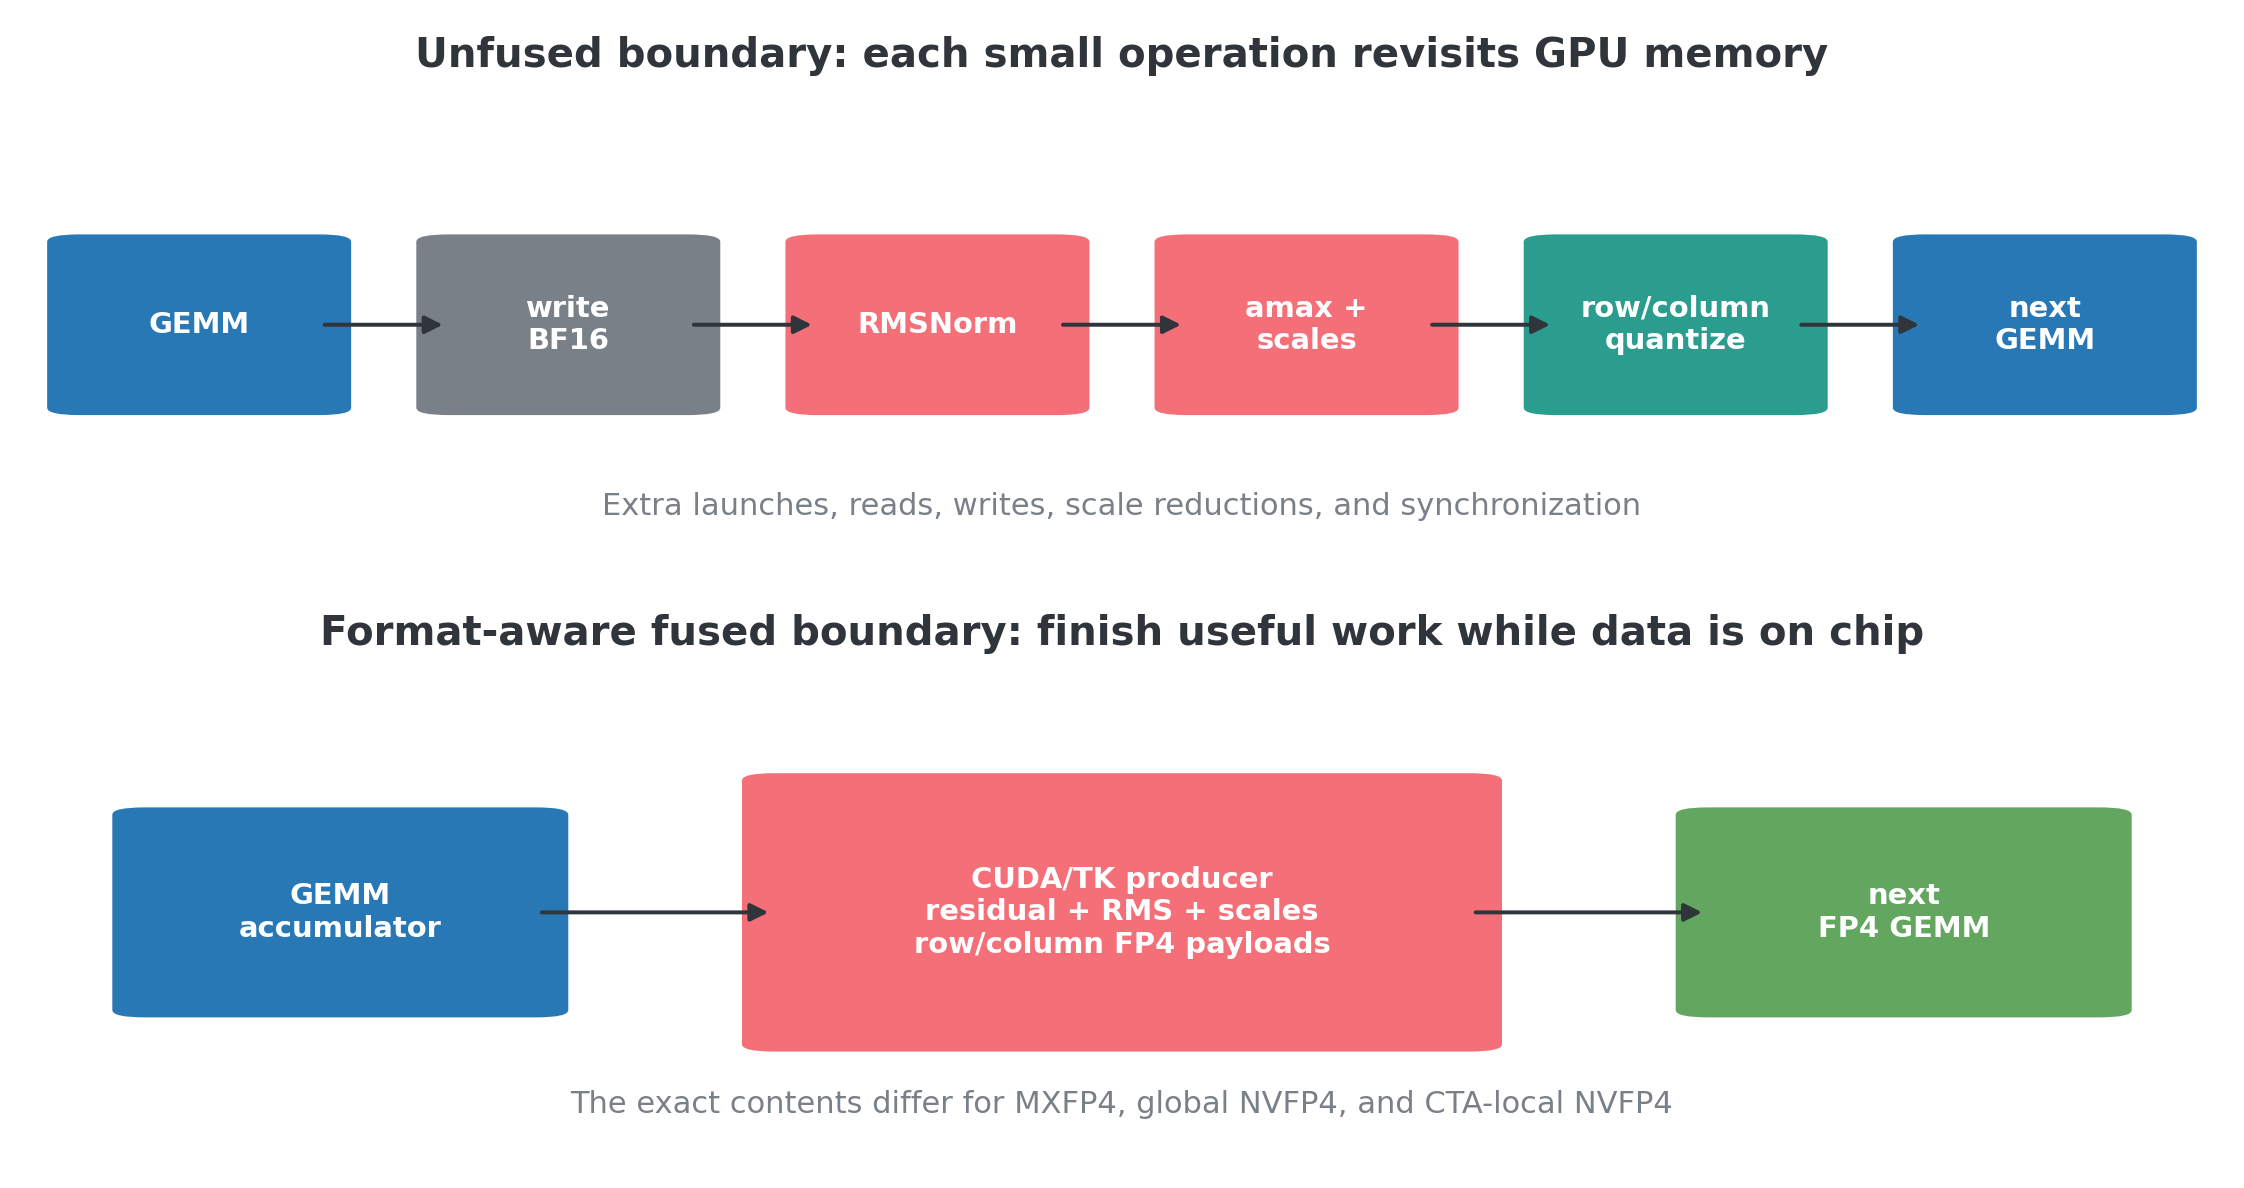
\includegraphics[width=0.93\textwidth]{figures/fp4_fusion_dataflow.png}
  \caption{Format-aware fusion treats normalization, scale production,
  physical layout, the consuming GEMM, and backward state as one execution
  boundary.}
  \label{fig:fusion-dataflow}
\end{figure}

We implement the fused tensor operations in CUDA and \tk{}
\cite{spector2024thunderkittens}. Following CODA's GEMM-plus-epilogue framing
\cite{guo2026coda}, an operation joins a boundary only when the next stage can
consume its output directly. A Llama block exposes four such boundaries:
root-mean-square normalization (RMSNorm) into the query/key/value (QKV)
projection, QKV into attention, the gated feed-forward network (FFN), and the
residual update into the next RMSNorm. Each has a corresponding backward
boundary.

\subsection{What is fused in a Llama block}

The system specializes four repeated Llama boundaries.  Table~\ref{tab:fusion-ledger}
states both the shared algebra and the format-dependent schedule.

\begin{table}[tbp]
  \centering
  \caption{High-level fusion ledger. ``Both views'' means the row and column
  representations required by Equations~\ref{eq:dgrad}
  and~\ref{eq:wgrad}.}
  \label{tab:fusion-ledger}
  \begin{tabularx}{\textwidth}{lYYY}
    \toprule
    Boundary & \mxfp{}-v4 & Global \nvfp{} v5 & \localcta{}-v4 \\
    \midrule
    RMSNorm $\rightarrow$ QKV
      & Row statistics, normalized value, local scales, and both views share a producer
      & Tensor amax starts with normalization; scale completion and layout are overlapped
      & Row/column tile outer scales and both views are emitted without a global barrier \\
    QKV $\rightarrow$ attention
      & Grouped Q/K/V GEMM; Q/K rotary position embedding (RoPE) is owned by the projection boundary
      & Same algebra with native NVFP4 payload/scale descriptors
      & Same algebra; GEMM epilogue applies the two outer corrections \\
    Gated FFN
      & W1/W3 scheduling plus sigmoid linear unit (SiLU)--gate output and the W2 input producer
      & Native 16-value quantization replaces generic TE-to-custom materialization
      & W2 Dgrad, SiLU derivative, and split W1/W3 backward representations are co-produced \\
    Residual $\rightarrow$ RMSNorm
      & Exact residual and row statistics are carried while next FP4 views are formed
      & Global-scale work is launched early rather than hidden in a nominal epilogue
      & K-invariant outer scales remain available through the consuming GEMM \\
    Backward layouts
      & One producer emits deterministic column payloads and row-SR payloads with checkpointed random state
      & One native producer emits 16-value hierarchical views and 2D-weight descriptors
      & One producer emits row/column E2M1, E4M3 per-block scales, and FP32 outer scales \\
    \bottomrule
  \end{tabularx}
\end{table}

The gated FFN illustrates why the boundary extends beyond a GEMM.
Writing W1 and W3 outputs to BF16, launching a separate SiLU--multiply, then
reading the result again to quantize W2's input spends bandwidth between every
large contraction. The fused path schedules the paired projections together
and emits W2's FP4 input with the SiLU--gate output. In backward, it combines
W2 Dgrad with the SiLU derivative and produces the representations consumed by
W1/W3 Dgrad and Wgrad. Exact BF16 values remain available where autograd
requires them; fusion changes data movement, not the model definition.

QKV follows the same principle. The normalized input producer emits the
format-specific representations consumed by the grouped projection, and the
Q/K projection applies RoPE and the required layout. Backward combines inverse
layout, RoPE, QKV gradient production, and the adjacent RMSNorm reduction when
their data dependencies align. Residual--RMSNorm retains the exact residual
and row statistics while producing the next quantized representations.

Scale work is scheduled by format. \mxfp{} reductions finish with each local
tile. Global \nvfp{} begins the tensor amax early so scale finalization can
overlap other work. \localcta{} removes that global dependency, but its two
outer scales must remain available through the full K reduction.
Figure~\ref{fig:format-execution-routes} summarizes these schedules.

\subsection{Depth-wise and operand-wise hybrids}

The \emph{depth-wise} hybrid assigns complete transformer blocks 1--27 to
\localcta{} and blocks 28--32 to \mxfp{}. Attention and FFN linears follow the
assigned block, so Fprop, Dgrad, and Wgrad never mix formats within one linear.
Both formats use orientation-consistent 2D weights and row-only gradient-data
SR; neither uses Hadamard preconditioning.

The \emph{operand-wise} hybrid instead chooses the format per contraction. A
same-state operator analysis found lower Dgrad error for \localcta{} than for
\mxfp{} in every measured layer and component. This motivates \mxfp{} for
Fprop and Wgrad and \localcta{} for Dgrad. The diagnostic and its scope are
reported in Section~\ref{sec:results} and
Appendix~\ref{app:dgrad-diagnostic}.

Concretely, every linear uses \mxfp{}-v4 for Fprop and Wgrad and
\localcta{}-v4 with row-data SR for Dgrad. One producer loads each BF16
gradient tile once and emits both the CTA-local row representation and the MX
column representation. The weight producer likewise loads BF16 $W$ once and
emits the MX forward view and the CTA-local Dgrad view.

We evaluate two Wgrad variants. The plain-H16 variant applies the same
16-value Hadamard mixing to $X$ and $dY$ with $D=I$, so it performs no sign
flips. The fixed-H32 variant applies the paired 32-value signed transform used
by the completed \mxfp{}+row-SR+fixed-H32 route. Neither variant transforms the
stored weight. Fprop, CTA-local Dgrad, weight encodings, row SR, output
projection, and loss retain the same numerical contract. Table~\ref{tab:gb200-throughput}
reports the two complete configurations; Appendix~\ref{app:implementation}
gives the exact sign mapping.

Every main custom route retains a BF16 output projection and compiled regular cross
entropy. Appendix~\ref{app:output-head} summarizes the low-precision output
heads that did not improve the end-to-end speed--numerics tradeoff.
\FloatBarrier
